\section{ConvKB: A Novel Embedding Model for Knowledge Base Completion Based on Convolutional Neural Network}
\subsection{研究背景与目的}

\begin{frame}[c]{Introduction}

\begin{block}{\small A Novel Embedding Model for Knowledge Base Completion Based on Convolutional Neural Network}
	\begin{itemize}
	    \item Author: Dai Quoc Nguyen, Tu Dinh Nguyen, Dat Quoc Nguyen, Dinh Phung
	    \item Lab: PRaDA Centre, Deakin University, Australia. The University of Melbourne, Australia.
	    \item Comments: NAACL 2018.
	\end{itemize}
\end{block}

\begin{block}{Abstract}
	\begin{itemize}
	    \item 基于卷积神经网络的模型能学习更丰富、更具表象力的Embedding,作者将它应用在了知识图谱的关系预测任务中。
	    \item 作者提出了一种1D卷积的方法同时作用于知识图谱的三元组上,用于同时捕捉实体和关系向量之间的交互关系,称作ConvKB。
	    \item ConvKB实验效果在多个数据集的效果和效率指标上均优于各Baseline。
	\end{itemize}
\end{block}

\end{frame}

\subsection{研究内容与方法}

\begin{frame}[c]{Background}

\begin{itemize}
    \item 知识图谱可以表示为$G=(E,R)$,其中$E$和$R$分别表示实体(节点)集合和关系(边)集合。对于知识图谱里的三元组$(h,r,t)$可以表示为两个实体节点$h$和$t\ (h, t \in E)$之间存在类型为$r\ (r\in R)$的边。\\ 
    \begin{center}
        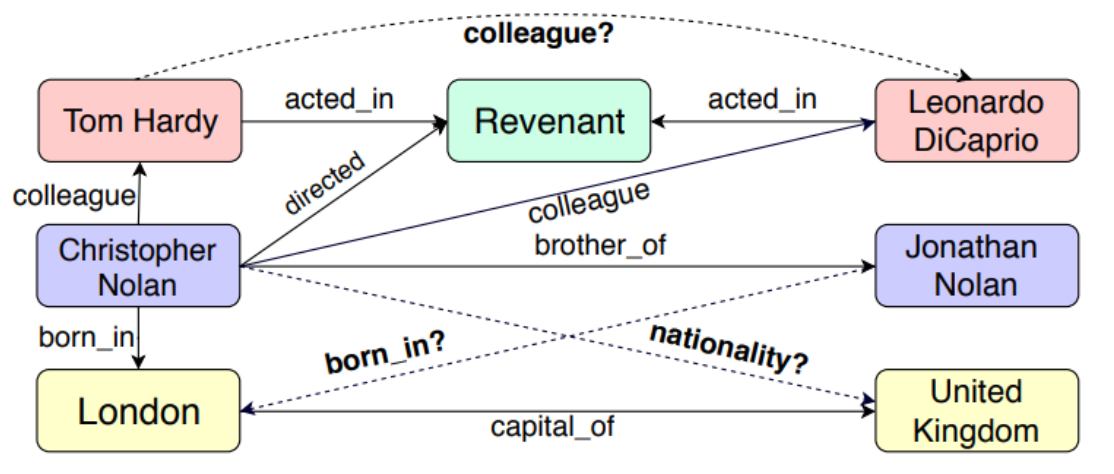
\includegraphics[width=8cm]{assets/1.png}
    \end{center}
    \item 表示学习模型:学习实体和关系的有效嵌入表示(Embedding),服务于下游任务。
    \item 关系预测模型:学习评分函数$f(\cdot)$,输入待预测三元组$(h,r,t)$,输出关于它的评分$f(h,r,t)$。评分规则取决于损失函数的设计。例如\texttt{MarginLoss}约束真实三元组分数要比负采样的虚假三元组分数高。
\end{itemize}

\end{frame}

\begin{frame}[c]{ConvKB - Architecture}

\begin{figure}
    \centering
    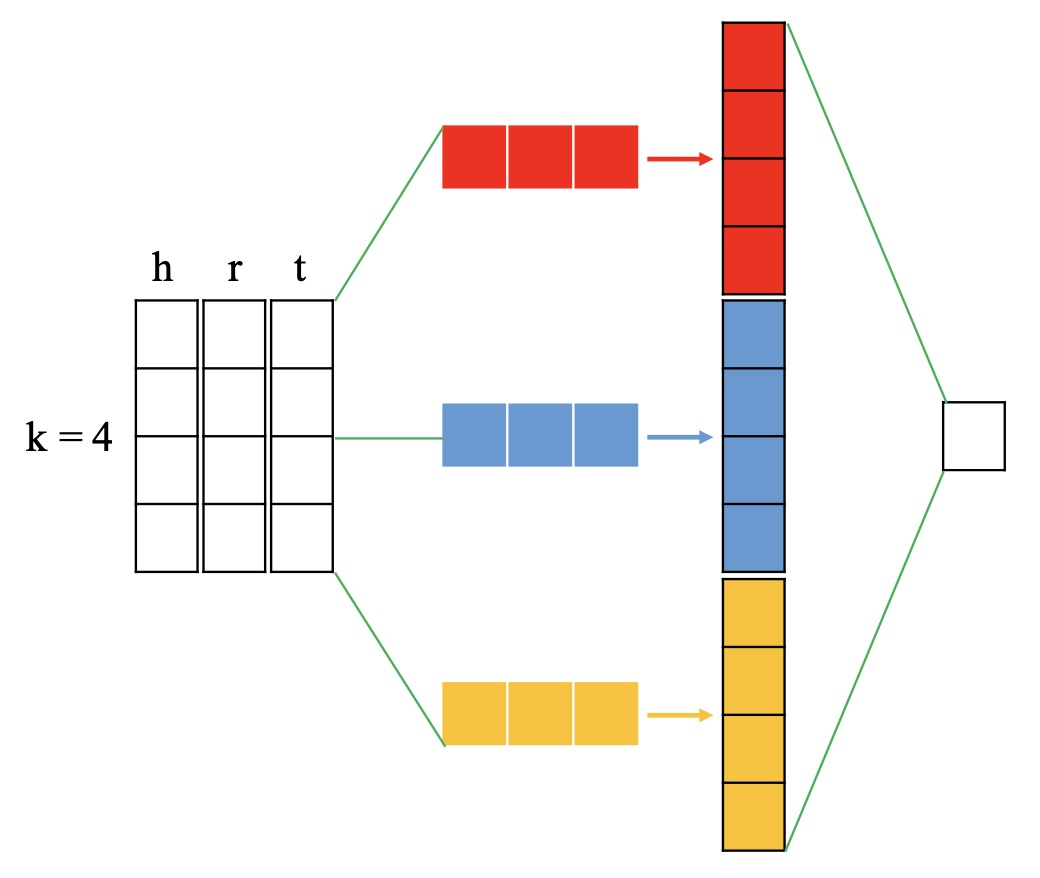
\includegraphics[width=4cm]{assets/7.png}
    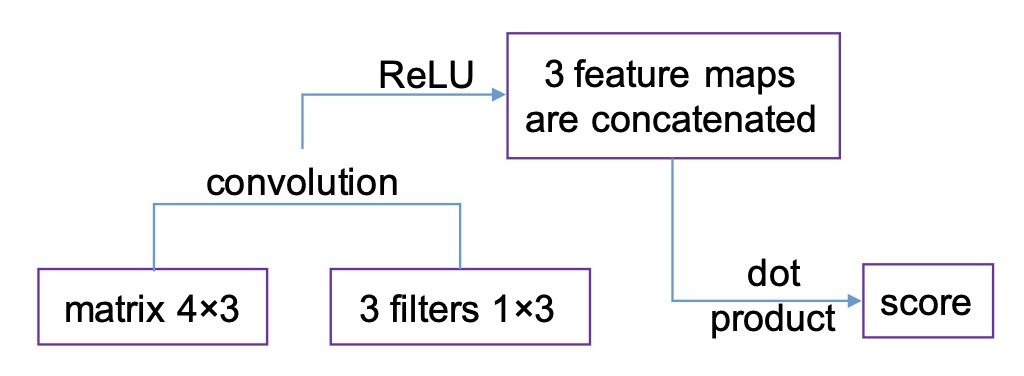
\includegraphics[width=5cm]{assets/8.png}
\end{figure}

\begin{itemize}
    \item 作者认为ConvE没有关注到三元组$(h,r,t)$是具有相同维度的整体存在,忽略元组作为整体这一全局信息。
    \item ConvKB将$(h,r,t)$三元组表示为为3列的矩阵,输送到卷积层使用多个卷积核进行卷积操作输出为若干的Feature map。接着,将它们拼接为一个单个的特征向量作为三元组卷积后的Embedding表示。最后,通过一个全连接层得到它的评分。
    \item 直观感受,将整体丢进去卷积,学习的交互信息更加丰富了。
\end{itemize}
    
\end{frame}

\begin{frame}[c]{ConvKB - Details}

\begin{itemize}
    \item 输入的三元组构成矩阵$\bm{A}=[\bm{v}_h,\bm{v}_r,\bm{v}_t]\in \mathbb{R}^{k\times 3}$,通过若干卷积核$\bm{\omega}=\{\omega^{(i)}\in \mathbb{R}^{1\times 3}\}$得到特征向量$\bm{v}=[v_1,v_2,\cdots,v_k]\in \mathbb{R}^k$,即$v_i=g(\bm{\omega\cdot A}_i+b)$,其中$b$是偏置单元,$g(\cdot)$是非线性函数(作者使用的激活函数为\texttt{ReLU})。
    \item 训练时按一定的比例进行负采样,在负采样时对于真实的三元组$(h,r,t)$随机将$h$和$t$替换为虚假的实体(作者使用的正负采样比例为$1:10$)。
    \item 损失函数使用\texttt{SoftMarginLoss},即$\mathcal{L}=\sum\limits_{(h,r,t)}\log(1+\exp(-l_{(h,r,t)}\cdot f(h,r,t)))+\frac{\lambda}{2}{\lVert \mathbf{w}\rVert}^2_2$,其中$l_{(h,r,t)}$为三元组的标签(对于真实的三元组置标签为$1$,负采样的假三元组置以$-1$),$f(\cdot)$为评分函数,$\lambda$为正则化的超参数。
\end{itemize}
    
\end{frame}


\subsection{实验结果与分析}

\begin{frame}[c]{ConvKB - Details}

\begin{itemize}
    \item 评分函数使用$f(h,r,t)=\texttt{concat}(g([\bm{v}_h,\bm{r},\bm{v}_t]*\Omega))\cdot \mathbf{W}$,其中$\Omega$和$W$均为可训练的网络参数,基于WN18RR和FB15k-237进行对比实验,在当时几乎可以做到state-of-the-art。
\end{itemize}

\begin{center}
    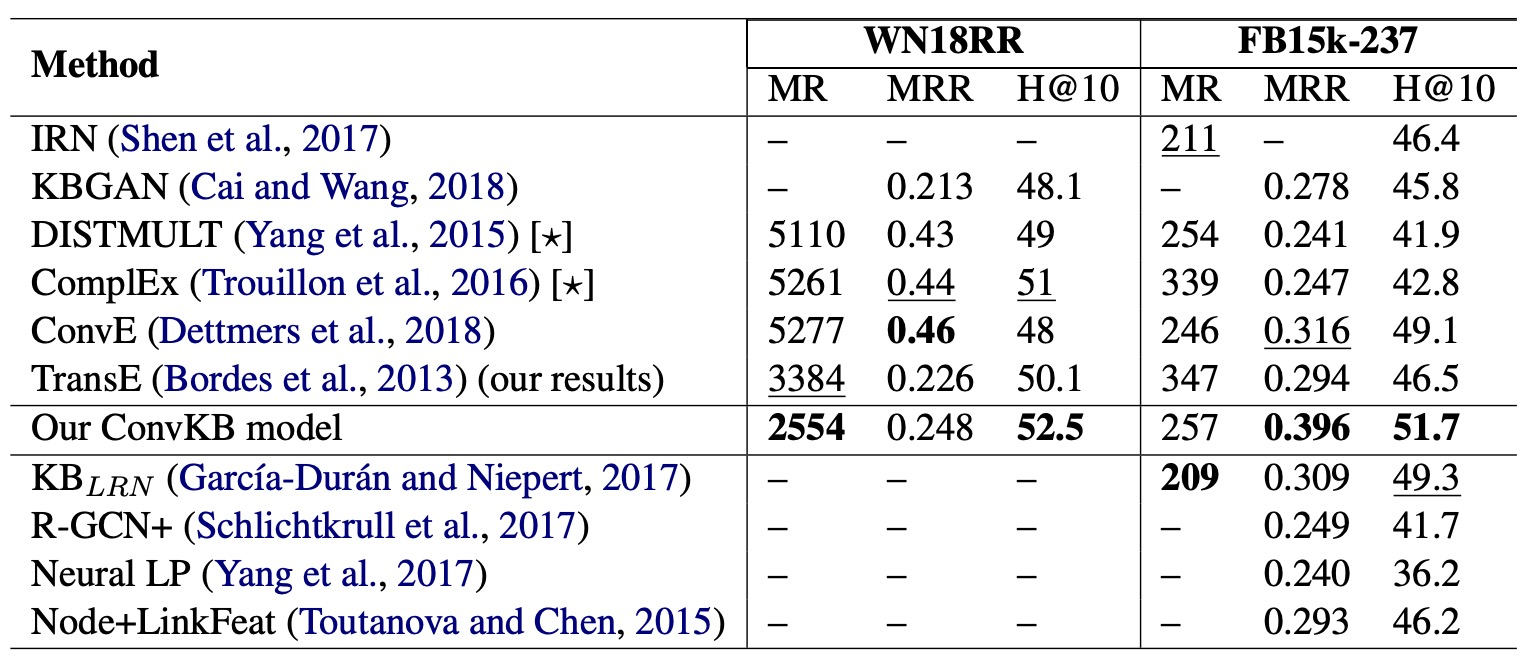
\includegraphics[width=13cm]{assets/9.png}
\end{center}

    
\end{frame}